\subsection{Model Fit}
\label{subsec:fit_results}

This section compares simulated data from our model with empirical data from Germany. We
look at observed infections, fatality rates,\comment[id=K]{should we include them?} the
spread of the B.1.1.7 mutation, vaccinations\comment[id=K]{We fit vaccinations in the
population by construction. Maybe this should go to a different section?} and rapid test
demand. Where available we do not only look at aggregated statistics but also analyze the
model fit for age groups and federal states.

% summary of the fit
Overall, our model achieves an excellent fit of the two waves of infections with few free
parameters (Figure~\ref{fig:aggregated_fit2}. As a result the effective replication
number is similar to that reported by the Robert Koch-Institut (see
Figure~\ref{fig:fit_r_effective}). This excellent fit is also achieved for most age
groups in Germany. The fit is also good for many German federal states even though our
synthetic population does not represent the differences in the distribution of age groups
and they only had a small weight in the optimization. Despite, the fact that the number
of performed rapid tests and their distribution in the population results endogenously
inside our model we fit the share of the population with at least a weekly rapid test
very well and err on the side of too few individuals that have ever done a rapid test.

% observed infections

\begin{figure}[ht]   % observed infections with single runs
  \centering
  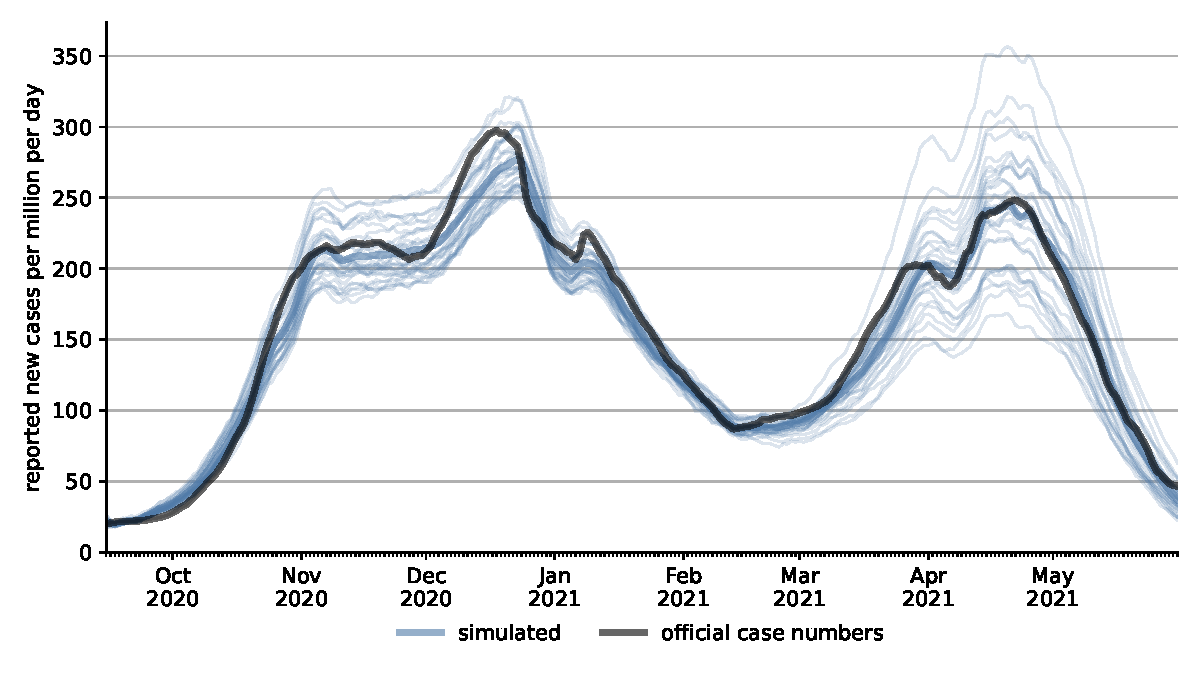
\includegraphics[width=\textwidth]{figures/results/figures/scenario_comparisons/combined_fit/full_new_known_case_with_single_runs}
  \caption{Fit Over the Full Simulation Time Frame with Single Simulation Runs}
  \floatfoot{\noindent \textit{Note:} The figure shows the weekly incidence rates per
  100,000 people for the reported simulated infections rates. The mean infection rate is
  the thick blue line. Single simulation runs are plotted in lighter and thinner lines.
  The official case numbers as reported by the Robert-Koch-Institut are plotted in black.
  The fit is overall very good. The higher the mean incidence and the stronger the growth
  the more variance there is between simulation runs. We averaged over 30 simulation
  runs.}
  \label{fig:aggregated_fit2}
\end{figure}


\textcolor{red}{...} High levels of infections often coincide with increased statistical
uncertainty, as for example in April and May.

\begin{figure}[ht]  % observed infections by age group
  \centering
  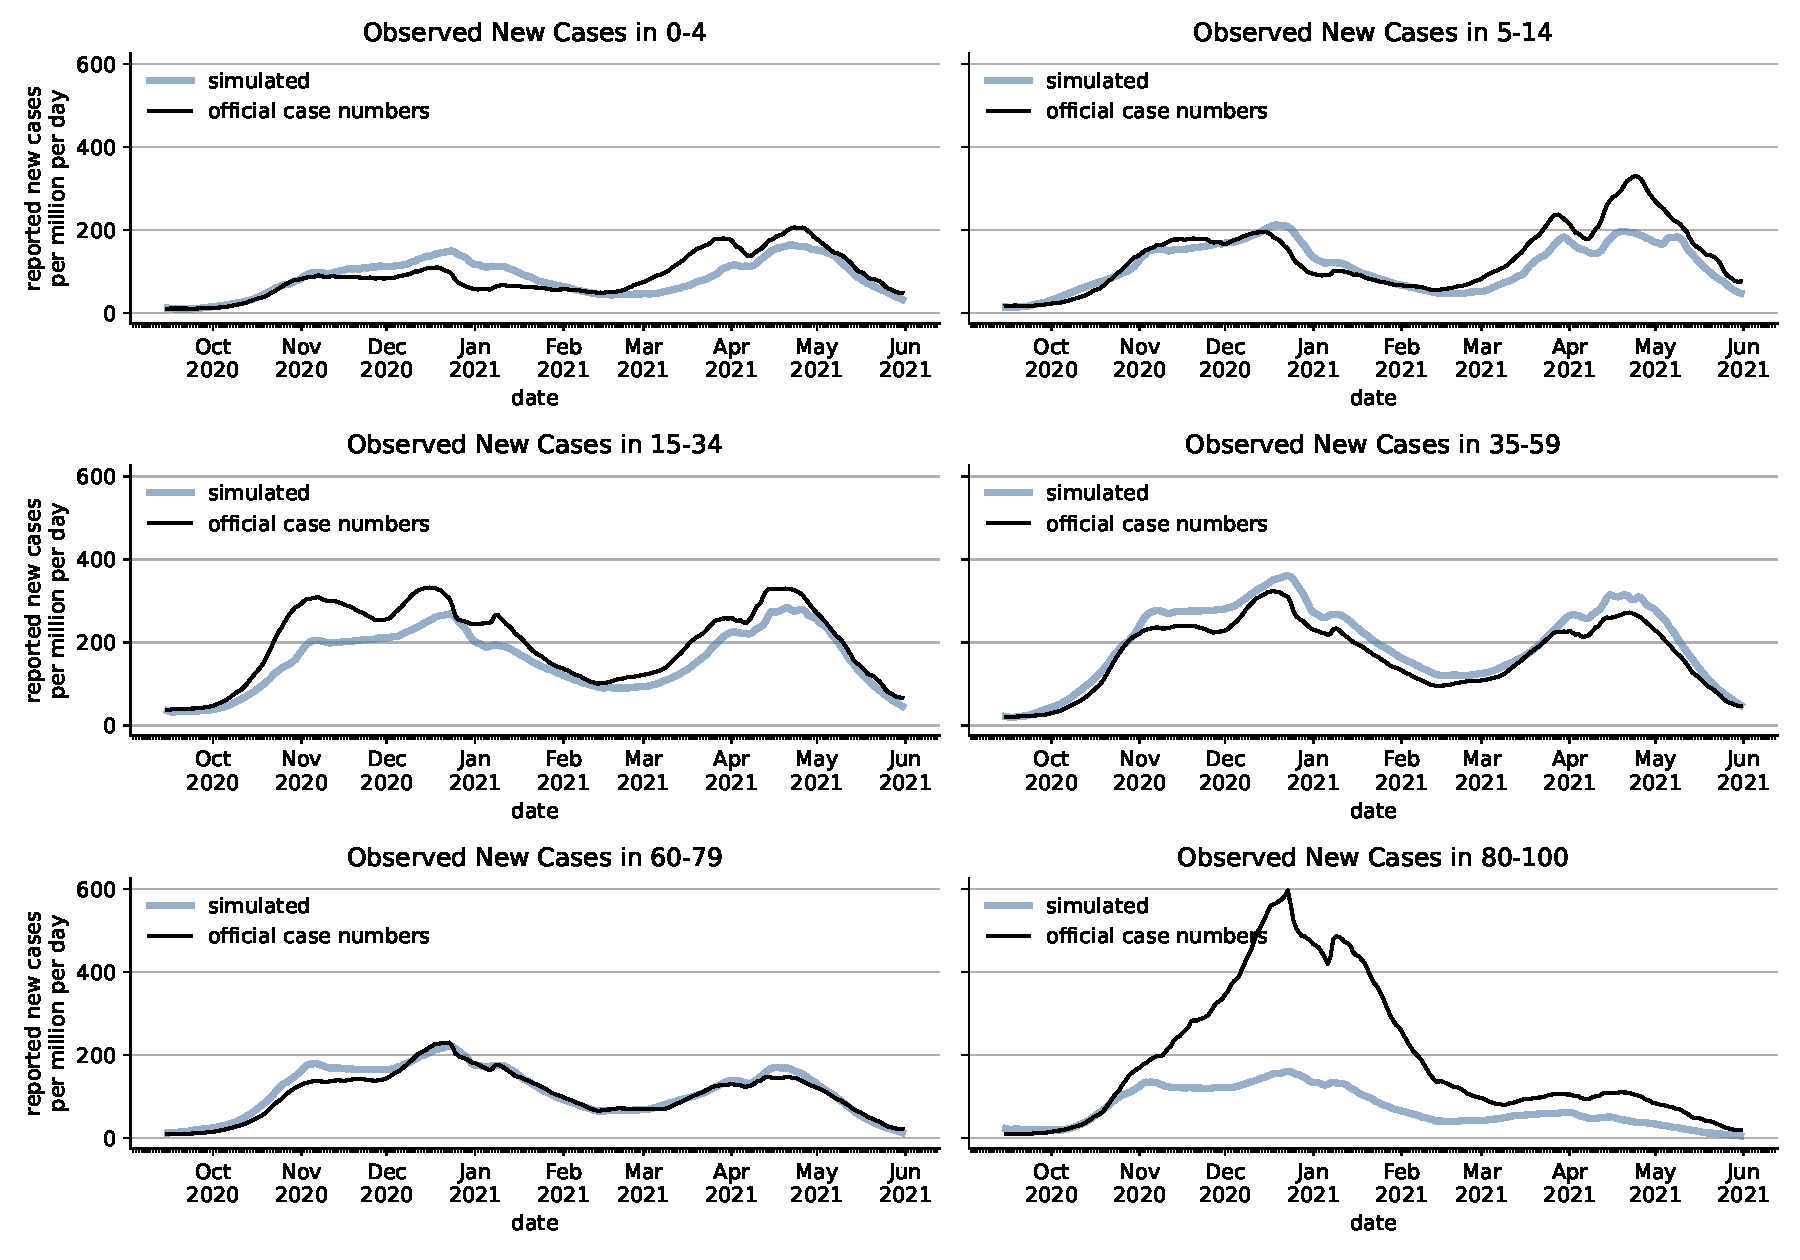
\includegraphics[width=\textwidth]{figures/results/figures/incidences_by_group/age_group_rki/full_combined_baseline_new_known_case}
  \caption{Simulated and Empirical Infections by Age Group}
  \floatfoot{\noindent \textit{Note:} The figure shows the weekly incidence rates per
  100,000 people for the reported versus the simulated infections rates for different age
  groups. The age group of individuals above 80 needs to be interpreted with caution
  because our synthetic population only includes private households, i.e. nursing homes
  are not represented in our model. They accounted for many cases and deaths in the
  winter of 2020 and many 80 to 100 year olds live in these facilities. However, the
  official data does not contain information on whether cases were nursing home
  inhabitants or not. We averaged over 30 simulation runs.}
  \label{fig:age_group_fit}
\end{figure}

\textcolor{red}{...} One important exception are the 80 to 100 year olds where we do not
fit the large number of cases in the winter of 2020/2021. This is because we do not model
nursing homes where a large fraction of this age group lives and a very large fraction of
cases in that age group occurred.


\begin{figure}[ht]   % observed infections by federal state
  \centering
  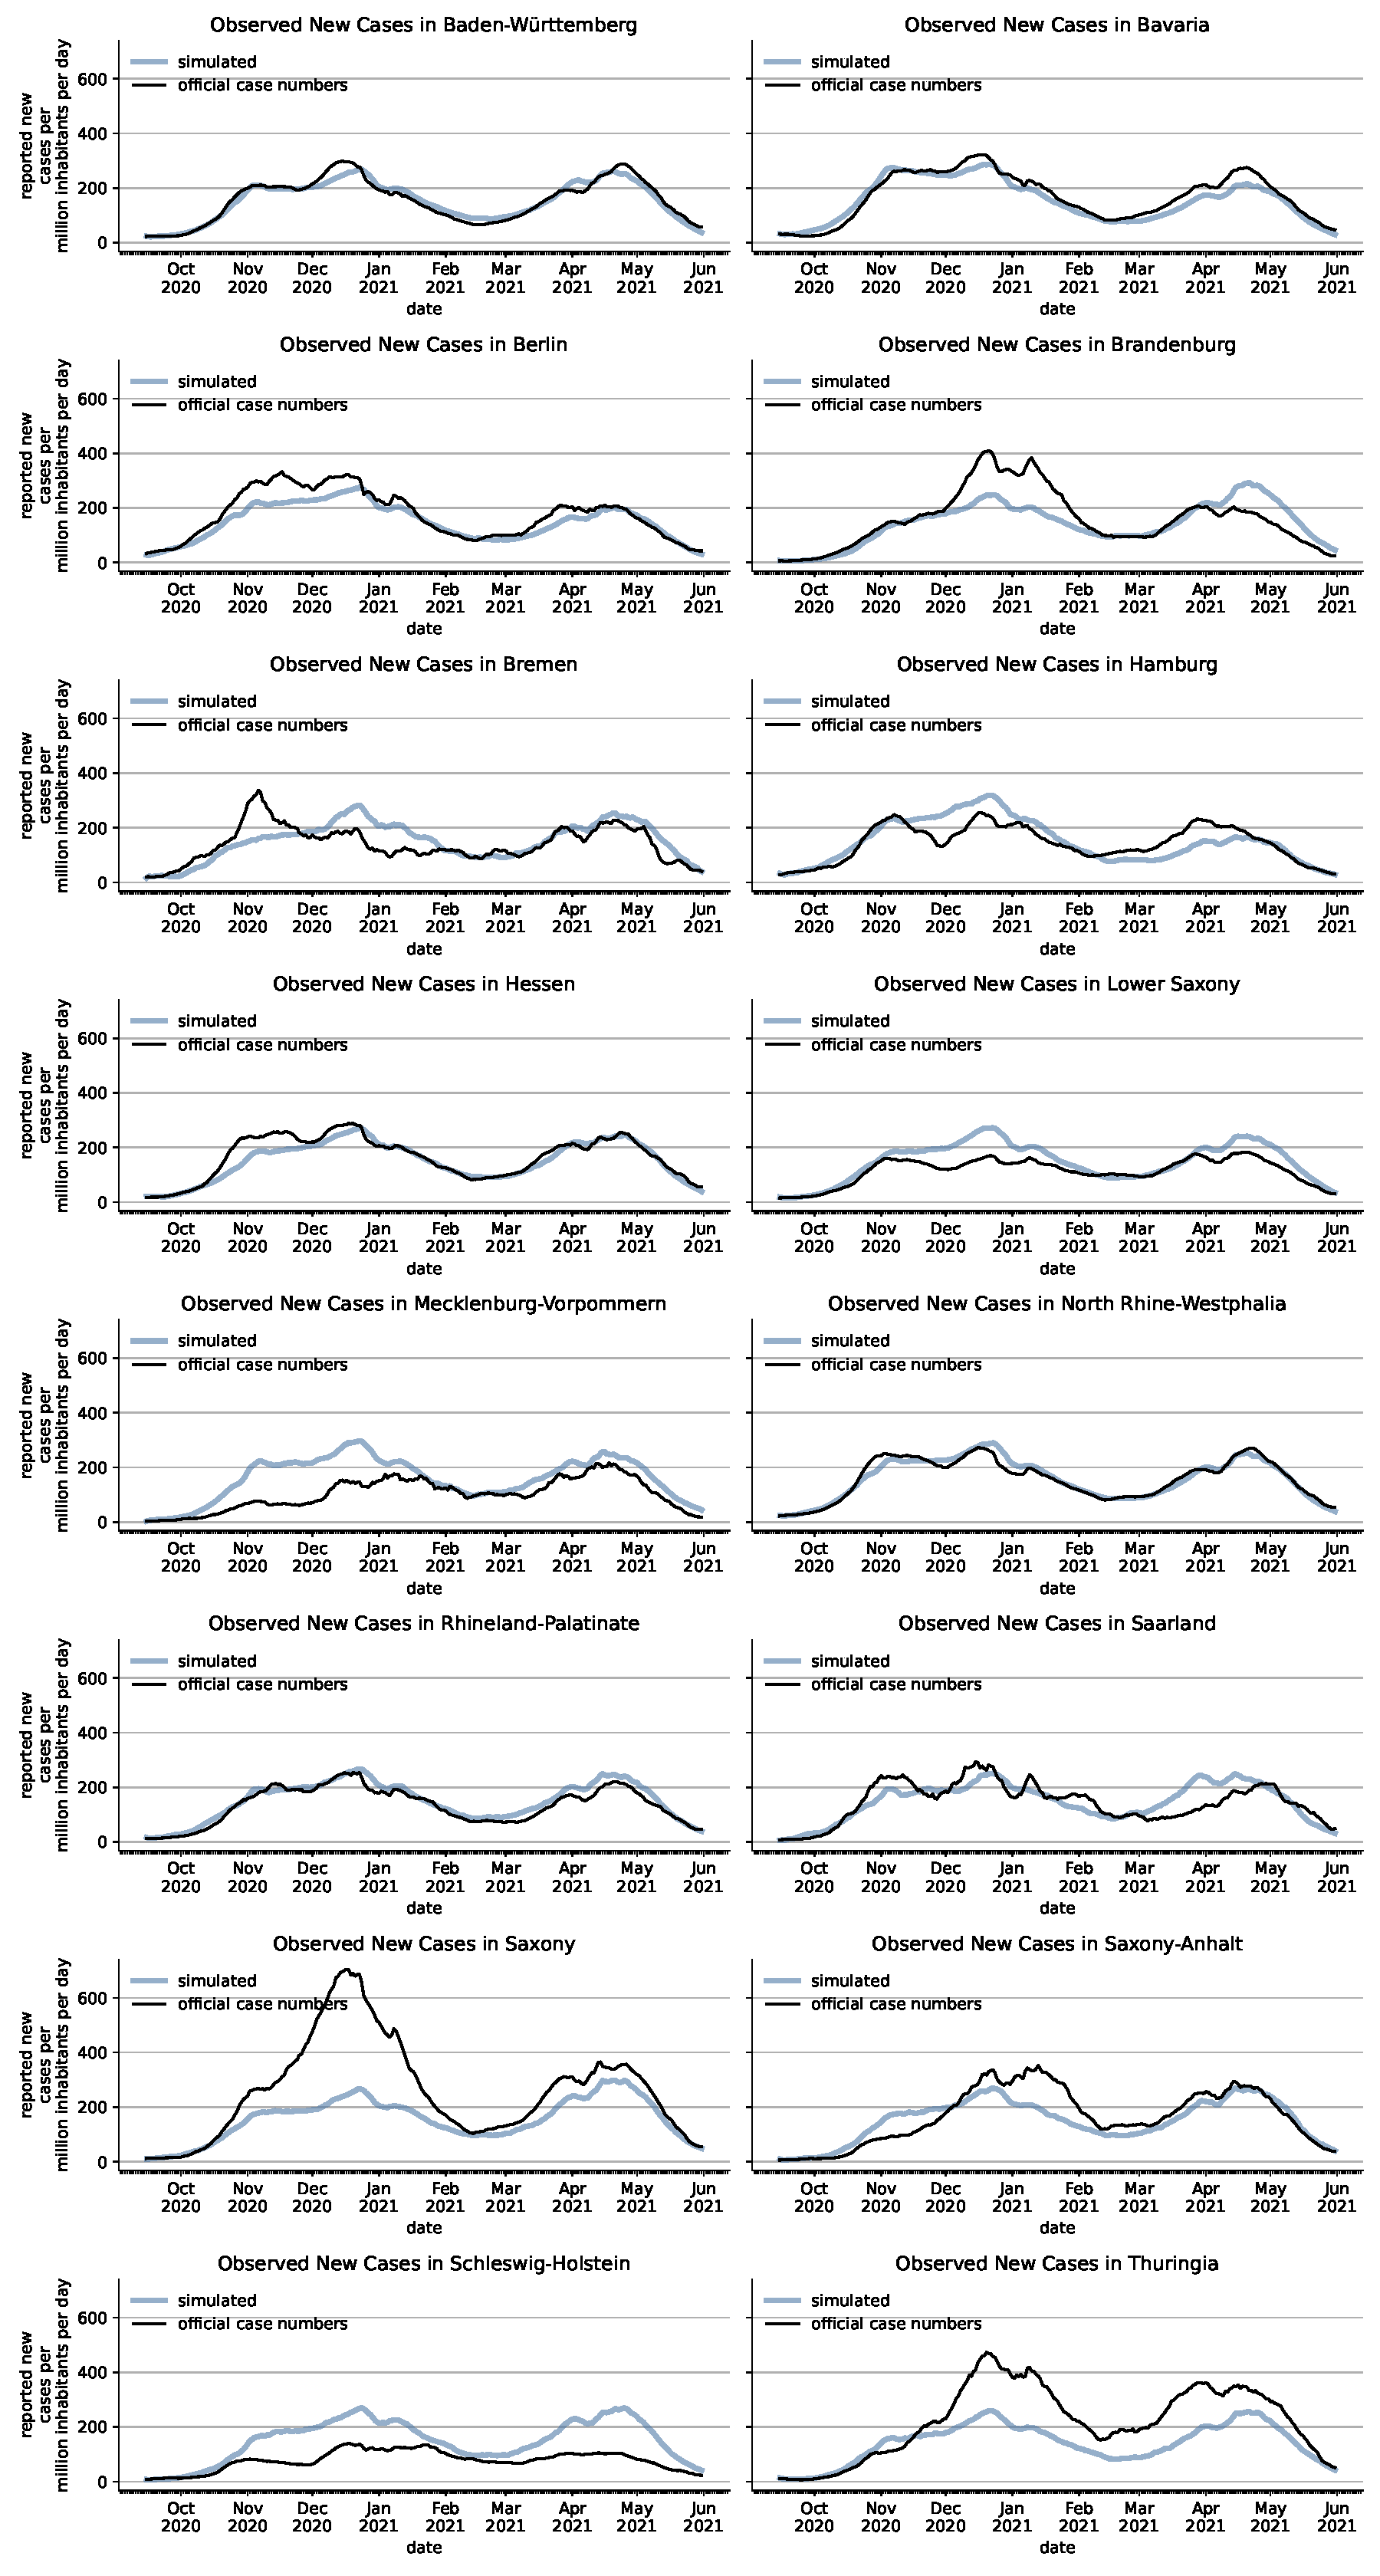
\includegraphics[height=0.95\textheight]{figures/results/figures/incidences_by_group/state/full_combined_baseline_new_known_case}
  \caption{Simulated and Empirical Infections by Federal State}
  \floatfoot{\noindent \textit{Note:} The figure shows the weekly incidence rates per
  100,000 people for the reported versus the simulated infections rates for different
  federal states. We averaged over 30 simulation runs.}
  \label{fig:state_fit}
\end{figure}

Our states are uniform with respect to their age distribution. \textcolor{red}{...}

Our fit of the effective replication number $R_t$ closely follows the values reported by
the RKI. \textcolor{red}{ldots}

\begin{figure}[ht]   % R effective
  \centering
  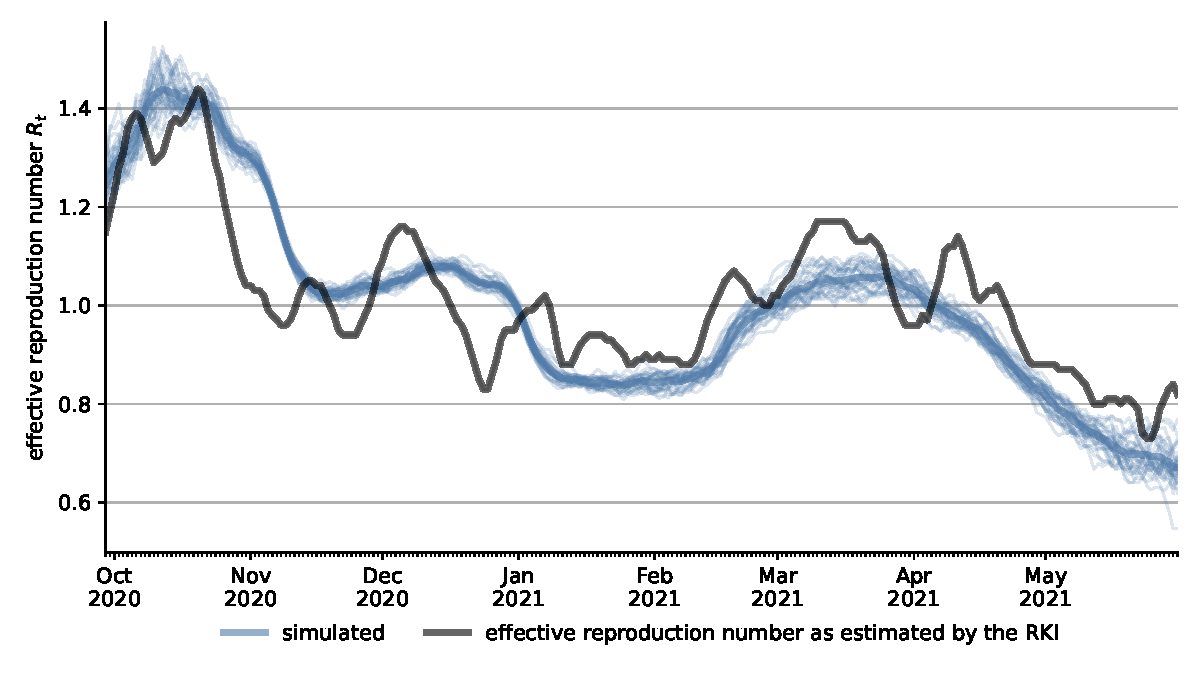
\includegraphics[width=\textwidth]{figures/results/figures/scenario_comparisons/combined_fit/full_r_effective_with_single_runs}
  \caption{Effective Replication Number $R_t$ in the Model and as Reported by the
  Robert-Koch-Institute}
  \floatfoot{\noindent \textit{Note:} The figure shows the effective replication number
  ($R_t$) as reported by the RKI and as calculated in our model. The $R_t$ gives the
  average number of new infections caused by one infected individual. The $R_t$ in our
  model broadly follows the $R_t$ reported by the RKI. Two trends stand out. Firstly, the
  RKI's $R_t$ drops faster in November. This could be due to a change in the testing
  policy that focused tests on the elderly when the second wave hit Germany and led to a
  decline in the overall share of detected cases. The second difference is from mid
  February to mid March where the RKI's reported $R_t$ increased more rapidly than that
  in our model. Here the opposite effect can be expected. During this time rapid tests
  increased strongly leading to more cases being detected. In the short term this leads
  an $R_t$ estimation that is based on detected cases to overestimate the replication
  number.}
  \label{fig:fit_r_effective}
\end{figure}


% fatality rates: MISSING


\begin{figure}[ht]   % Share B.1.1.7
  \centering
  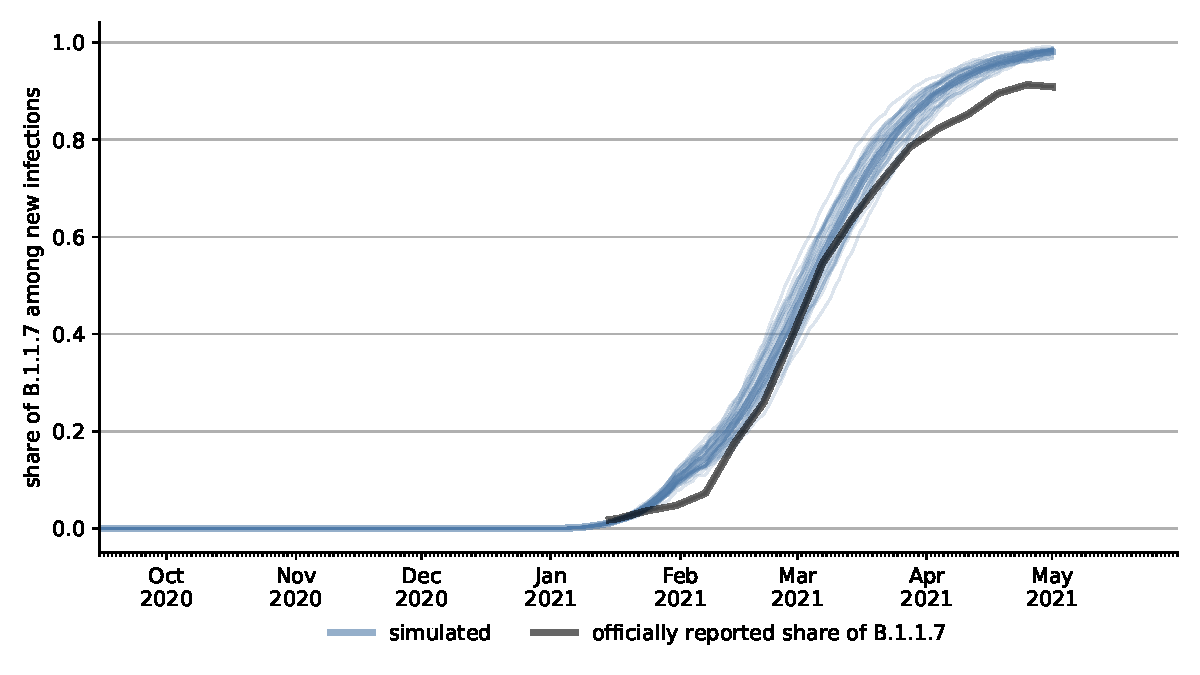
\includegraphics[width=\textwidth]{figures/results/figures/scenario_comparisons/combined_fit/full_share_b117_with_single_runs}
  \caption{Share of B.1.1.7 in the Model and as Reported by the Robert-Koch-Institute}
  \floatfoot{\noindent \textit{Note:} The figure shows the share of B.1.1.7 as
  reported by the RKI and as calculated in our model. We only introduce a few cases over
  the cause of January. From then B.1.1.7 takes over endogenously through its increased
  infectiousness. We model no other features of B.1.1.7. At most we introduce 0.75 cases per 100,000 inhabitants.}
  \label{fig:fit_share_b117}
\end{figure}


\begin{figure}[ht]   % fit of vaccinations
  \centering
  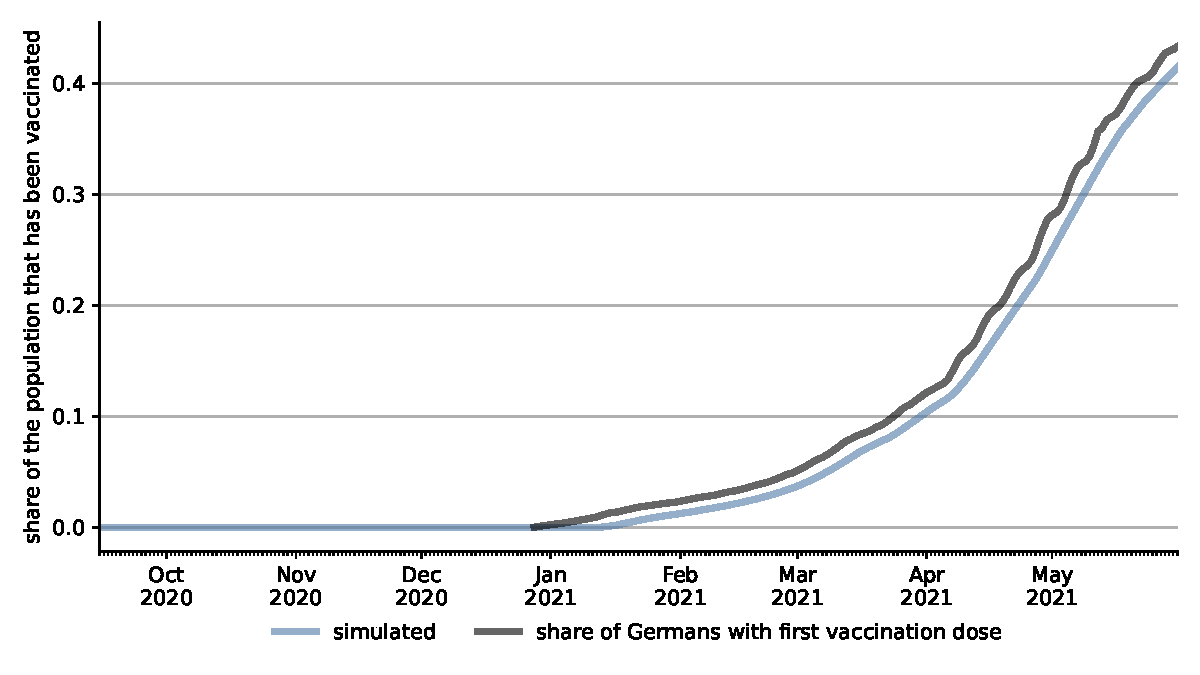
\includegraphics[width=\textwidth]{figures/results/figures/scenario_comparisons/combined_fit/full_ever_vaccinated}
  \caption{Share of Vaccinated Individuals}
  \floatfoot{\noindent \textit{Note:} The figure shows the rate of individuals that are
  vaccinated in our synthetic population versus in the general German population. Note
  that we excluded the vaccinations that were given to nursing homes, approximately the
  first percent of the German population that were vaccinated. Overall, our model covers
  a time frame that goes from zero vaccinated individuals to a state where over 40\% of
  the population are vaccinated. Our vaccinations work imperfectly but we do not model
  different vaccines nor do we distinguish between first and second shot.}
  \label{fig:fit_vaccinations}
\end{figure}


\begin{figure}[ht]     % rapid test demand
    \centering
    \caption{Share of Individuals With Rapid Tests}
    \label{fig:share_ever_rapid_test}
    \begin{subfigure}{.55\textwidth}
        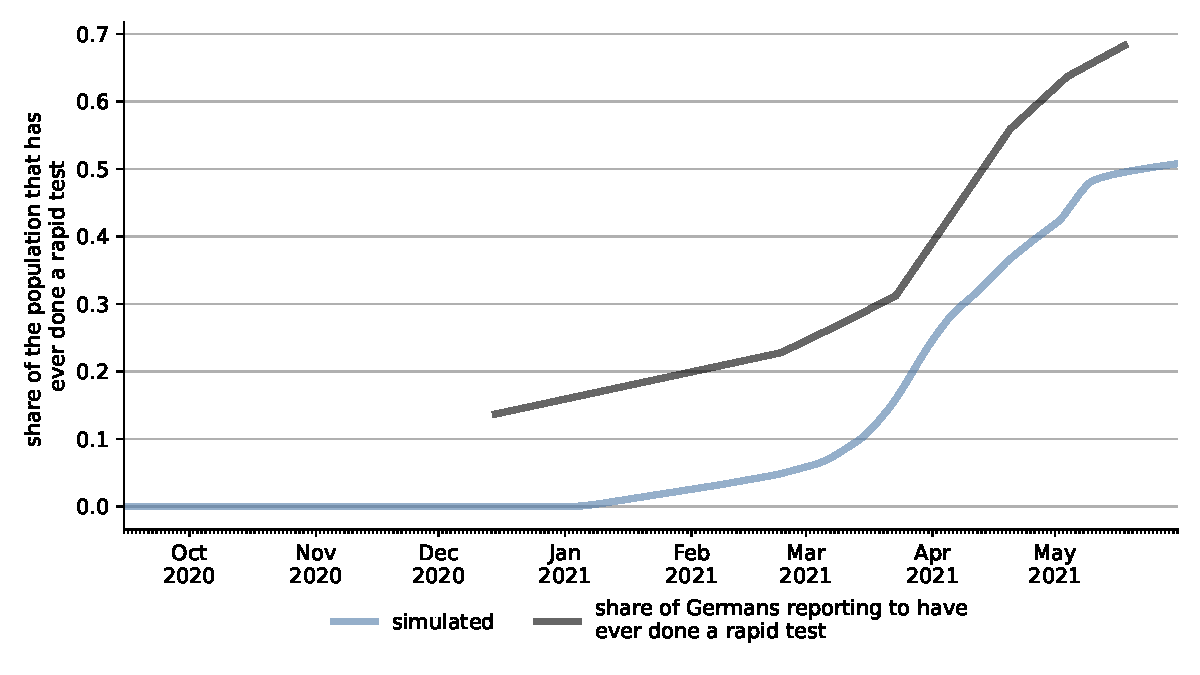
\includegraphics[width=0.9 \textwidth]{figures/results/figures/scenario_comparisons/combined_fit/full_share_ever_rapid_test}
        \caption{Share of Individuals That Have Ever Done a Rapid Test}
    \end{subfigure}%
    \begin{subfigure}{.55\textwidth}
        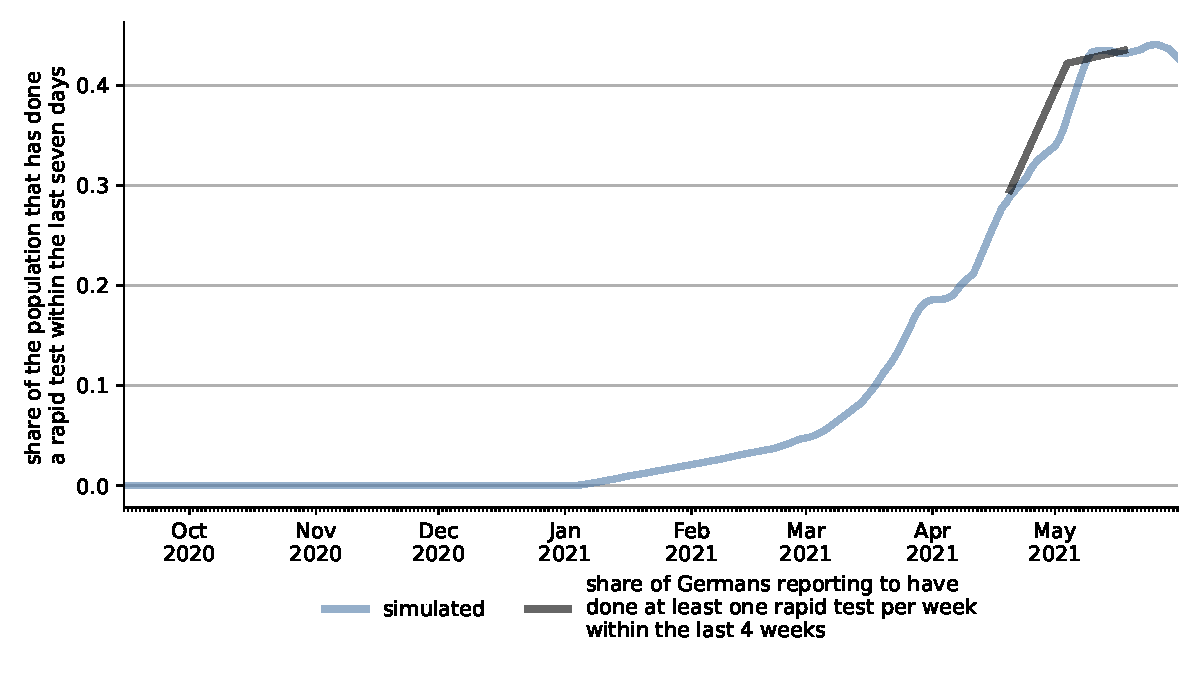
\includegraphics[width=0.9 \textwidth]{figures/results/figures/scenario_comparisons/combined_fit/full_share_rapid_test_in_last_week}
        \caption{Share of Individuals Having Done a Rapid Test in the Last Week}
    \end{subfigure}
    \label{fig:share_rapid_test_last_week}
    \floatfoot{\noindent \textit{Note:} The figure compares the share of individuals who
        have ever done a rapid test or done a rapid test within the last week in our
        simulations to the shares reported in the
        \href{https://projekte.uni-erfurt.de/cosmo2020/web/topic/wissen-verhalten/80-schnelltests/}{COVID-19
        Snapshot Monitoring Survey}. The left panel compares the share of individuals who
        have ever done a rapid test. The right panel compares the share of individuals
        who have done a rapid test within the last seven days in our simulation compared
        to the share reporting to have done at least weekly rapid tests in the last four
        weeks in the COSMO survey. Overall our calibration of rapid tests are slightly
        conservative. The overall share is below that in the study. We fit the share of
        weekly tests quite exactly. However, the study only covers adults while our share
        also includes children who are tested very regularly when attending school.}
\end{figure}



\FloatBarrier

